\documentclass[10pt]{amsart}
\usepackage{amsmath,amsfonts}
\usepackage{setspace}
\usepackage{tkz-euclide}
\usepackage{nopageno}
\usepackage{soul}
\usepackage{tikz}
\usepackage{xcolor}
\usepackage{hyperref} 


%%%%%%%%%%%% Tikz commands for HMM
\tikzstyle{state}=[shape=circle,draw=black!50,minimum size = 2cm,node distance = 5cm]
\tikzstyle{observation}=[shape=rectangle,draw=black!50]
\tikzstyle{lightedge}=[<-,dotted]
\tikzstyle{mainstate}=[state,thick]
\tikzstyle{mainedge}=[<-,thick]

%Style section
\setlength{\textheight}{10in}
\setlength{\textwidth}{6.5in}
\hoffset=-0.75in
\voffset=-1in
% \pagestyle{plain}
% \setlength{\topmargin}{0in}
% \setlength{\headsep}{0in}
% \setlength{\oddsidemargin}{0in}
% \setlength{\evensidemargin}{0in}

%% packages for  code
\usepackage{listings}
\usepackage{color}

\definecolor{dkgreen}{rgb}{0,0.6,0}
\definecolor{gray}{rgb}{0.5,0.5,0.5}
\definecolor{mauve}{rgb}{0.58,0,0.82}

\lstset{frame=tb,
  language=Python,
  aboveskip=3mm,
  belowskip=3mm,
  showstringspaces=false,
  columns=flexible,
  basicstyle={\small\ttfamily},
  numbers=none,
  numberstyle=\tiny\color{gray},
  keywordstyle=\color{blue},
  commentstyle=\color{dkgreen},
  stringstyle=\color{mauve},
  breaklines=true,
  breakatwhitespace=true,
  tabsize=3
}

%%%%%%%%%%%%%%%%%%%%%%%%%%%%%%
%%% My shorthands commands %%%
%%%%%%%%%%%%%%%%%%%%%%%%%%%%%%
\newcommand{\bff}{{\bf f}}
\newcommand{\bfx}{{\bf x}}
\newcommand{\bfb}{{\bf b}}
\newcommand{\bfu}{{\bf u}}
\newcommand{\bfv}{{\bf v}}
\newcommand{\bfh}{{\bf h}}
\newcommand{\bfy}{{\bf y}}
\newcommand{\bfe}{{\bf e}}
\newcommand{\bfz}{{\bf z}}
\newcommand{\bfw}{{\bf w}}
\newcommand{\bfr}{{\bf r}}
\newcommand{\bfL}{{\bf L}}
\newcommand{\bfX}{{\bf X}}
\newcommand{\bfY}{{\bf Y}}
\newcommand{\bfE}{{\bf E}}
\newcommand{\bfA}{{\bf A}}
\newcommand{\bfI}{{\bf I}}
\newcommand{\bfone}{{\mathbf{1}}}

\DeclareMathOperator*{\argmin}{arg\,min}


\begin{document}

\noindent
{Math 118 \hfill Homework Assignment 5 Spring 2020}
%\vskip 0.1truein
\bigskip
\begin{quote}\emph{This is your fifth and final homework assignment. I strongly encourage you to typeset it using the LaTeX template provided. It is due by Friday, March 13th. After class on Wednesday I will add a question on Pagerank.} \\
\end{quote}
\hrulefill
\vskip 0.1truein

\vspace{0.3cm}
\begin{center}
{\bf The following questions are on constrained optimization.}
\end{center}
\vspace{0.3cm}

\begin{enumerate}

\item The non-negative least squares problem is:
$$
\bfx^{*} = \argmin_{\bfx\in\mathbb{R}^{d}: \ \bfx \geq 0} \|A\bfx - \bfb\|_{2}^{2}
$$
In this question we will discuss using projected gradient descent (PGD) for this problem. Note that we can write this as:
$$
\bfx^{*} = \argmin_{\bfx\in\mathcal{X}} f(\bfx)  \quad \text {where } \mathcal{X} = \left\{\mathbb{R}^{d}: \ \bfx \geq 0\right\} \text{ and } f(\bfx) = \|A\bfx - \bfb\|_{2}^{2}
$$
Recall that PGD is defined by the iteration $\bfx_{k+1} = \mathcal{P}_{\mathcal{X}}\left(\bfx_k - \alpha\nabla f(\bfx_k)\right)$. For this particular region $\mathcal{X}$, the projection is defined component-wise as:
$$
\left[\mathcal{P}_{\mathcal{X}}(\bfv)\right]_{i} = \left\{\begin{array}{cc} v_i & \text{ if } v_i \geq 0 \\ 0 & \text{ otherwise} \end{array}\right. 
$$
Suppose that:
$$
A = \left[\begin{matrix} 0.5377 & -0.8622 \\ 1.8339 & 0.3188 \\ -2.2588 & 1.3077 \end{matrix}\right] \quad \text{ and } \bfb = \left[\begin{matrix} -0.4336 \\ 0.3426 \\ 0.5163 \end{matrix} \right]
$$
Given $\bfx_0 = \left[\begin{matrix} 0 & 0 \end{matrix}\right]^{\top}$ use PGD to find $\bfx_1,\bfx_2$ and $\bfx_3$.  You may do this by hand, or you may use a computer. Take the step size, $\alpha$, to be $0.01$. {\em Recall that in a previous homework assignment we established that ${\nabla f(\bfx) = 2A^{\top}\left(A\bfx - \bfb\right)}$}.

\bigskip
\noindent\textbf{Answer:} 
\\~\\$\bfx_{k+1} = \mathcal{P}_{\mathcal{X}}\left(\bfx_k - \alpha\nabla f(\bfx_k)\right)$ where $\bfx_0=\left[\begin{matrix} 0 & 0 \end{matrix}\right]^{\top}$, $\alpha=0.01$, with ${\nabla f(\bfx)}$ and $\left[\mathcal{P}_{\mathcal{X}}(\bfv)\right]_{i}$ defined above.
\\~\\For simplicity, I used the following python code to complete calculations. Note that each function below is defined to represent mathematical functions like ${\nabla f(\bfx)}$ and $\left[\mathcal{P}_{\mathcal{X}}(\bfv)\right]_{i}$

\begin{lstlisting}
// PGD.py
import numpy as np

A = np.array([[0.5377, -0.8622],
              [1.8339, 0.3188],
              [-2.2588, 1.3077]], np.float64)

b_trans = np.array([-0.4336, 0.3426, 0.5163], np.float64)
b = np.transpose(b_trans)

a = 0.01
x_0 = np.transpose(np.array([0, 0]))


def main():
   x_1 = x_k_plus_one(x_0)
   x_2 = x_k_plus_one(x_1)
   x_3 = x_k_plus_one(x_2)

   print("x_1: ", x_1)
   print("x_2: ", x_2)
   print("x_3: ", x_3)



def x_k_plus_one(x_k):
   return P_x(x_k - a * grad_f(x_k))

def grad_f(x_k):
   C = np.matmul(A, x_k) - b
   return np.matmul(2*np.transpose(A), np.transpose(C))

def P_x(v):
   for j, i in enumerate(v):
      if i >= 0:
         continue
      else:
         v[j] = 0
   return v

if __name__ == "__main__":
    main()
""" ########## Output ##########
x_1:  [0.         0.02316473]
x_2:  [0.         0.04514569]
x_3:  [0.         0.06600338]
"""
\end{lstlisting}
\bigskip Through this process, I have calculated that $\bfx_1 = \left[\begin{matrix} 0 & 0.02316473 \end{matrix}\right]^{\top}$, $\bfx_2 = \left[\begin{matrix} 0 & 0.04514569 \end{matrix}\right]^{\top}$, and $\bfx_3 = \left[\begin{matrix} 0 & 0.06600338 \end{matrix}\right]^{\top}$, as desired. If you'd like to run/test the code, it can be found \href{https://github.com/broeib/Math-118/blob/master/PGD.py}{\textcolor{blue}{here}}
\bigskip
\bigskip
\item Consider the constrained least squares problem:
\begin{equation*}
\bfx^{*} = \argmin_{\bfx\in\mathbb{R}^{d}: \ \|\bfx\|_2 \leq 1}\|A\bfx - \bfb\|_{2}^{2} 
\label{eq:Constrained_LS}
\end{equation*}

The constraint $\|\bfx\|_2\leq 1$ serves to ensure that the entries in the solution are not too large. Instead of solving this directly, one can consider the {\em penalty method} to approximately solve the problem. This means solving:
\begin{equation*}
\bfx^{\#} = \argmin_{\bfx\in\mathbb{R}^{d}} f(\bfx) = \|A\bfx - \bfb\|_{2}^{2} + \gamma \|\bfx\|_{2}^{2}
\end{equation*}
This problem is also called {\em ridge regression}. Let's also define:
$$
\bfx^{\dagger} = \argmin_{\bfx\in\mathbb{R}^{d}}\|A\bfx - \bfb\|^{2}_{2}
$$

\begin{enumerate}
	\item As $\gamma\to 0$ do you expect $\bfx^{\#}\to \bfx^{*}$ or $\bfx^{\#}\to \bfx^{\dagger}$? Explain your answer.
	\item For intermediate values of $\gamma$, do you expect $\bfx^{\#}\approx \bfx^{*}$ or $\bfx^{\#} \approx \bfx^{\dagger}$? Explain your answer?
	\item As $\gamma\to \infty$ what will happen to $\bfx^{\#}$? Explain your answer. 
\end{enumerate} 

\bigskip
\noindent\textbf{Answer:} 
\\~\\\textbf{(a)} As $\gamma\to 0$, I expect $\bfx^{\#}\to \bfx^{\dagger}$. This is because as $\gamma\to 0$, $\lim_{\gamma\to 0} \gamma \|\bfx\|_{2}^{2}=0$, so $\bfx^{\#}$ becomes $\argmin_{\bfx\in\mathbb{R}^{d}} f(\bfx) = \|A\bfx - \bfb\|_{2}^{2} + 0$ which is identical to $\bfx^{\dagger}$. The reason I do \textbf{not} expect $\bfx^{\#}\to \bfx^{*}$ is because $\bfx^{*}$ has the restriction of $\|\bfx\|_2\leq 1$, which will restrict solutions from $\bfx^{\#}$.
\\~\\~\\\textbf{(b)} For intermediate values of $\gamma$, I expect $\bfx^{\#}\rightarrow\bfx^*$. For intermediate values, we want to minimize the $\|\bfx\|_2^2$ term, and if $\|\bfx\|_2\leq 1$, then $\gamma\|\bfx\|_2^2\rightarrow 0$ for increasing gamma. If $\|\bfx\|_2 > 1$, then $\gamma\|\bfx\|_2^2\rightarrow\infty$. For our minimization problem, we will have the constraint where $\|\bfx\|_2\leq 0$, which is given by $\bfx^*$.
\\~\\~\\\textbf{(c)} As $\gamma\to\infty$, I expect $\bfx^{\#}$ to approach 0. If we want to find the value of $\bfx$ that minimizes $\argmin_{\bfx\in\mathbb{R}^{d}} f(\bfx) = \|A\bfx - \bfb\|_{2}^{2} + \gamma \|\bfx\|_{2}^{2}$, a large value of $\gamma$ will make the term $\|\bfx\|_{2}^{2}$ very large, so we need an infinitesimally small value for $\|\bfx\|_2^2$ to compensate.

\vspace{0.3cm}
\begin{center}
{\bf The following questions are on dynamic programming.}
\end{center}
\vspace{0.3cm}

\item Consider the following variant of the knapsack problem. Suppose that the Math 118 midterm consists of $5$ problems, worth $5$, $10$, $20$, $25$, $30$ and $35$ points respectively. However, the test is only out of $50$ points. You may attempt as many of the problems as you like, and your instructor will grade all of them and choose the subset of problems whose totals add up to less than or equal to $50$ giving you the best possible score.  Suppose you attempt all five questions. In what follows, $p_{i}$ represents the points achieved on the $i$-th question, while $t_i$ represents the total points available on the $i$-th question.
$$
p_1 = 4, t_1 = 5 \quad p_2 = 3, t_2 = 10 \quad p_3 = 17, t_3 = 20 \quad p_4 = 20, t_4 = 25 \quad p_5 = 30, t_5 = 35 
$$
Use dynamic programming to determine the optimal subset of questions, and your maximum achievable score. {\em (This is essentially the knapsack problem with $B = 50$, $s_i= t_i$ and $v_i = p_i$. Hint: Consider increasing the size of the ``knapsack'' in increments of $5$)}. Your answer should include the dynamic programming table you construct as part of the algorithm.
\bigskip
\\\noindent\textbf{Answer:} I was having trouble inserting an image into LaTeX document, so with the professor's permission I decided to save my images for (3) and (4) online and link to them. Here is my link to (3): \href{https://imgur.com/a/Az0rko4}{\textcolor{blue}{link}}. As you can see from back-propogation in the image, the optimal subset of problems is problem 1, problem 3, and problem 4.
\item Use dynamic programming to find the longest common subsequence between $\mathbf{X} = GGATCGT$ and $\bfY = CGAGCTT$.  Your answer should include the dynamic programming table you construct as part of the algorithm. \\
Here is my link to (4): \href{https://imgur.com/a/813ZH2J}{\textcolor{blue}{link}}. As you can see, all optimal substring lengths are 4 and the one I showed with my back-propogation is GGCT.

\item Consider the dishonest casino problem modeled by the Hidden Markov Model (HMM) given below. 
\begin{figure}[h!]
\begin{center}
\resizebox{6cm}{4cm}{%
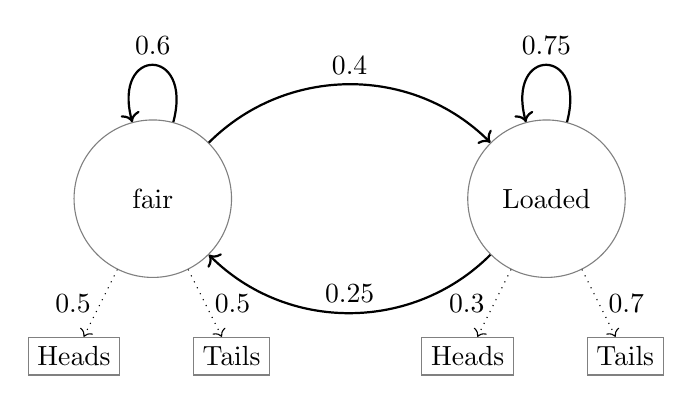
\begin{tikzpicture}
\node [state] (fair) at (0,0) {fair}
	edge[mainedge,loop above,distance = 1cm] node [above]{0.6} (fair);
\node [state, right of=fair] (not_fair) {Loaded}
	edge[mainedge,->,bend right = -45] node [above]{0.25} (fair)
	edge[mainedge,<-,bend right = 45] node [above]{0.4} (fair)
	edge[mainedge,loop above,distance = 1cm] node [above]{0.75} (not_fair);

\node [observation, below of = fair, node distance = 2cm, xshift = - 1cm] {Heads}
	edge [lightedge, <-] node [left] {0.5} (fair);
\node [observation, below of = fair, node distance = 2cm, xshift =  1cm] {Tails}
	edge [lightedge, <-] node [right] {0.5} (fair);
\node [observation, below of = not_fair, node distance = 2cm, xshift = - 1cm] {Heads}
	edge [lightedge, <-] node [left] {0.3} (not_fair);
\node [observation, below of = not_fair, node distance = 2cm, xshift =  1cm] {Tails}
	edge [lightedge, <-] node [right] {0.7} (not_fair);

\end{tikzpicture}
}
\end{center}
\end{figure}
Suppose we observe the sequence of emissions $\mathbf{Y}_6 = HTHTTT$ {\em (this is this same sequence we worked with in class)}. Use Viterbi's algorithm to find the most probable sequence of hidden states. (Here, the hidden states are of course ``F'' and ``L''). Assume an initial distribution of $\mathbb{P}[x_1 = F] = 1$ and $\mathbb{P}[x_1 = L] = 0$. Your answer should include the dynamic programming table you construct as part of the algorithm.

\bigskip
\noindent\textbf{Answer:} 
\\~\\$k=1$:
\\$f(F,1)=P(H|F)*P(F)=0.5*1=0.5$
\\$f(L,1)=P(H|L)*P(L)=0.3*0=0$
\\~\\$k=2$:
\\$f(F,2)=P(T|F)*max\left\{\begin{array}{c} 0.6f(F, 1) \\ 0.25f(L,1)\end{array}\right.=0.5*max\left\{\begin{array}{c} 0.3 \\ 0\end{array}\right.=0.15$
\\$f(L,2)=P(T|L)*max\left\{\begin{array}{c} 0.4f(F, 1) \\ 0.75f(L,1)\end{array}\right.=0.7*max\left\{\begin{array}{c} 0.2 \\ 0\end{array}\right.=0.14$
\\~\\$k=3$:
\\$f(F,3)=P(H|F)*max\left\{\begin{array}{c} 0.6f(F, 2) \\ 0.25f(L,2)\end{array}\right.=0.5*max\left\{\begin{array}{c} 0.09 \\ 0.035\end{array}\right.=0.045$
\\$f(L,3)=P(H|L)*max\left\{\begin{array}{c} 0.4f(F, 2) \\ 0.75f(L,2)\end{array}\right.=0.3*max\left\{\begin{array}{c} 0.06 \\ 0.105\end{array}\right.=0.0315$
\\~\\$k=4$:
\\$f(F,4)=P(T|F)*max\left\{\begin{array}{c} 0.6f(F, 3) \\ 0.25f(L,3)\end{array}\right.=0.5*max\left\{\begin{array}{c} 0.027 \\ 0.0189\end{array}\right.=0.0135$
\\$f(L,4)=P(T|L)*max\left\{\begin{array}{c} 0.4f(F, 3) \\ 0.75f(L,3)\end{array}\right.=0.7*max\left\{\begin{array}{c} 0.018 \\ 0.024\end{array}\right.=0.0165$
\\~\\$k=5$:
\\$f(F,5)=P(T|F)*max\left\{\begin{array}{c} 0.6f(F, 4) \\ 0.25f(L,4)\end{array}\right.=0.5*max\left\{\begin{array}{c} 0.0081 \\ 0.0041\end{array}\right.=0.00405$
\\$f(L,5)=P(T|L)*max\left\{\begin{array}{c} 0.4f(F, 4) \\ 0.75f(L,4)\end{array}\right.=0.7*max\left\{\begin{array}{c} 0.0054 \\ 0.0124\end{array}\right.=0.00866$
\\~\\$k=6$:
\\$f(F,6)=P(T|F)*max\left\{\begin{array}{c} 0.6f(F, 5) \\ 0.25f(L,5)\end{array}\right.=0.5*max\left\{\begin{array}{c} 0.00243 \\ 0.002165\end{array}\right.=0.001215$
\\$f(L,6)=P(T|L)*max\left\{\begin{array}{c} 0.4f(F, 5) \\ 0.75f(L,5)\end{array}\right.=0.7*max\left\{\begin{array}{c} 0.00162 \\ 0.006495\end{array}\right.=0.0045465$

\begin{table}[h]
\centering
\begin{tabular}{|l|l|l|l|l|l|l|} 
\cline{2-7}
\multicolumn{1}{l|}{} & k=1 & k=2  & k=3    & k=4    & k=5     & k-6        \\ 
\hline
                      & H   & T    & H      & T      & T       & T          \\ 
\hline
F                     & 0.5 & 0.15 & 0.045  & 0.0135 & 0.00405 & 0.001215   \\ 
\hline
L                     & 0   & 0.14 & 0.0315 & 0.0165 & 0.00866 & 0.0045465  \\
\hline
\end{tabular}
\end{table}
\bigskip
\bigskip
With these probabilities, the most likely states from $k=1$ to $k=6$ is FLLLLL, respectively. To figure out the back-propogation, I started at the bottom right corner and saw which value from $max\left\{\begin{array}{c} 0.4f(F, 5) \\ 0.75f(L,5)\end{array}\right.$ was larger. Since $0.006495>0.001215$, I knew that the state before is also L. I repeated this process and I ended up with FLLLLL.
\vspace{0.5cm}
\begin{center}
{\bf The following questions, still to be added, are on PageRank.}
\end{center}
\vspace{0.3cm}


\item In this question you will verify some things that were claimed, but not proven, in Lecture 22. The notation is as used in those slides.
\begin{enumerate}
	\item Verify that $\displaystyle P_{ij} = \frac{(A^{\top})_{ij}}{d^{\text{out}}_{j}}$
	\item Check that if $P$ is column stochastic, then so is $\tilde{P}$. {\em Remark: there was a minor typo in the definition of $\tilde{P}$ given in class. It should be:}
	$$
	\tilde{P} = \alpha P + (1-\alpha)\frac{1}{n}\mathbf{1}\mathbf{1}^{\top}
	$$	
	{\em Note the factor of $\frac{1}{n}$. Without this, $\tilde{P}$ will not be column-stochastic.}
\end{enumerate}
\bigskip
\noindent\textbf{Answer:} 
\\~\\\textbf{(a)} $\displaystyle P_{ij}=\sum_{k=1}^{n} \left(A^{\top}\right)_{ik}\left(D^{out}\right)_{kj}^{-1}$
\\~\\$=\left(A^{\top}\right)_{ij}\left(D^{out}\right)_{jj}^{-1}$
\\~\\$=\frac{\left(A^{\top}\right)_{ij}}{d_j^{out}}$
\\~\\\textbf{(b)} $\tilde{P} = \alpha P + (1-\alpha)\frac{1}{n}\mathbf{1}\mathbf{1}^{\top}$:
\\~\\$\displaystyle \sum_{i=1}^{n}\tilde{P_{ij}}=\sum_{i=1}^{n}\left(\alpha P_{ij}+\left(1-\alpha\right)\frac{1}{n}\textbf{11}^{\top}_{ij}\right)$
\\~\\$\displaystyle=\sum_{i=1}^{n}\left(\alpha P_{ij}\right)+\left(1-\alpha\right)\frac{1}{n}\sum_{i=1}^{n}\left(\textbf{11}^{\top}_{ij}\right)$
\\~\\$\displaystyle=\sum_{i=1}^{n}\left(\alpha P_{ij}\right)+\left(1-\alpha\right)\frac{1}{n}n$
\\~\\$\displaystyle=\alpha\sum_{i=1}^{n}\left(P_{ij}\right)+\left(1-\alpha\right)(1)$
\\~\\$=\alpha(1)+\left(1-\alpha\right)=1$
\\~\\Thus, if $P$ is column-stochastic, $\tilde{P}$ is also column-stochastic.
\\
\item  Consider the directed graph given below:

\begin{figure}[h]
%\includegraphics[width = 0.25\textwidth]{MarkovModel.pdf}
\end{figure}

\begin{enumerate}
	\item Write down the adjacency matrix $A$ for this directed graph. Is $A$ reducible or irreducible?\\
	\bigskip
	\noindent\textbf{Answer:} $\left[\begin{matrix}  & 1 & 2 & 3 & 4 \\ 1 & 0 & 1 & 0 & 0 \\ 2 & 1 & 0 & 0 & 0\\ 3 & 1 & 0 & 0 & 1 \\ 4 & 1 & 1 & 1 & 0\end{matrix}\right]$, $A=\left[\begin{matrix} 0 & 1 & 0 & 0 \\ 1 & 0 & 0 & 0\\ 1 & 0 & 0 & 1 \\1 & 1 & 1 & 0\end{matrix}\right]$. 
	\\~\\A is reducible because it is not strongly connected. For instance, if you start at vertex 1, there is no path to vertex 3 or 4.
	
	\item Compute the matrix $\tilde{P}$ we defined in class, for $\alpha = 0.95$. {\em And use the definition of $\tilde{P}$ given in (6.b)} \\
	\\\noindent\textbf{Answer:}
	\\$\tilde{P} = \alpha P + (1-\alpha)\frac{1}{n}\mathbf{1}\mathbf{1}^{\top}$
	\\~\\$=0.95P+(1-\alpha)\frac{1}{4}\mathbf{1}\mathbf{1}^{\top}$
	\\~\\$=\left[\begin{matrix} 0 & 0.95 & 0.475 & 0.3167 \\ 0.95 & 0 & 0 & 0.3167\\ 0 & 0 & 0 & 0.3167 \\0 & 0 & 0.475 & 0\end{matrix}\right]\left[\begin{matrix} 0.0125 & 0.0125 & 0.0125 & 0.0125 \\ 0.0125 & 0.0125 & 0.0125 & 0.0125\\ 0.0125 & 0.0125 & 0.0125 & 0.0125 \\0.0125 & 0.0125 & 0.0125 & 0.0125\end{matrix}\right]$
	\\~\\$=\left[\begin{matrix} 0.0125 & 0.9625 & 0.4875 & 0.329166 \\ 0.9625 & 0.0125 & 0.0125 & 0.329166\\ 0.0125 & 0.0125 & 0.0125 & 0.329166 \\0.0125 & 0.0125 & 0.4875 & 0.0125\end{matrix}\right]$
	\\\item Implement the power method, using MATLAB or Python, and use it to compute the leading eigenvector, $\bfv_1$, of $\tilde{P}$. {\em You may want to play with different numbers of iteration of the power method, as well as different initial $\bfv$. You should also compare the approximation to $\bfv_1$ you get from power method with the true leading eigenvector, obtainable using the {\tt eig} command in MATLAB}  \\
	\\\noindent\textbf{Answer:}
	\\~\\Below is my code for doing the power method in python:
	\begin{lstlisting}
//power_method.py
import numpy as np

P = np.array([[0, 1, 1/2, 1/3],
              [1, 0, 0, 1/3],
              [0, 0, 0, 1/3],
              [0, 0, 1/2, 0]], np.float64)
P_tilda = np.array([[0.0125, 0.9625, 0.4875, 0.329166],
                    [0.9625, 0.0125, 0.0125, 0.329166],
                    [0.0125, 0.0125, 0.0125, 0.329166],
                    [0.0125, 0.0125, 0.4875, 0.0125]])
def main():
   NUM_PRODUCTS = 10000
   v = np.random.rand(4, 1)
   for i in range(NUM_PRODUCTS):
      v = np.matmul(P_tilda, v)
   two_norm = np.linalg.norm(v)
   for j, i in enumerate(v):
      v[j] = (i / two_norm)
   print(v)
   print("\n\n", np.matmul(P_tilda, v))
   print("\n\n", np.linalg.eig(P_tilda)[1])
if __name__ == "__main__":
    main()
    
""" ########## Output ##########
[[0.70992482]
 [0.70297196]
 [0.02854335]
 [0.03197579]]


 [[0.70992479]
 [0.70297193]
 [0.02854334]
 [0.03197579]]


 [[ 7.09924823e-01  7.07106781e-01  4.16505334e-01 -3.15039459e-01]
 [ 7.02971957e-01 -7.07106781e-01  5.74692633e-01  1.82658761e-01]
 [ 2.85433455e-02  1.87022614e-18 -4.45533866e-01 -5.89027970e-01]
 [ 3.19757894e-02 -1.30644783e-17 -5.45665885e-01  7.21409708e-01]]

"""
	\end{lstlisting}
	Based on my results, my computed $\bfv_1=\left[\begin{matrix} 0.70992479 \\ 0.70297193 \\ 0.02854335 \\ 0.03197579 \end{matrix} \right]$. 
	\\~\\You can also see that in the first column of my output of $np.linalg.eig(P\_tilda)[1]$, my result is the same as the calculated first eigenvector of $\tilde{P}$.
	\\~\\If you'd like to run/test the code, it can be found \href{https://github.com/broeib/Math-118/blob/master/Problem_7.py}{\textcolor{blue}{here}}
	
	\item Using $\bfv_1$, rank the 4 vertices of this graph.
	\\\noindent\textbf{Answer:}
	\\~\\$\bfv_1=\left[\begin{matrix} 0.70992479 \\ 0.70297193 \\ 0.02854335 \\ 0.03197579 \end{matrix} \right]$. 
	\\~\\The ranks of the 4 vertices correspond to the respective sizes of the elements of $\bfv_1$ to one another. In other words, element 1 of $\bfv_1$ is the "rank" of vertex one, element 2 of $\bfv_1$ is the "rank" of vertex two, etc. Therefore, the rank of the 4 vertices are as follows: 
	\\~\\vertex 1 $>$ vertex 2 $>$ vertex 4 $>$ vertex 3. 
\end{enumerate}
\end{enumerate}


\end{document}